\chapter{Operating Systems Developments}
\section{Plan 9 Port to Blue Gene /L and /P}
\subsection{Large Pages}
Blue Gene   processors use software-loaded TLBs. A TLB manages the virtual to physical mapping for a single page, which 
in both Linux and Plan~9 is 4096 bytes. The processors support more than just one page size, in multiples of 4, from 1024 bytes to 1 Gbyte (with a few sizes missing). 
The CNK 
features 1 Mbyte TLBs, and benefits from reduced TLB fault interrupts. 

We extended Plan~9 to support larger TLBs. In order to measure the improvement we used the strid3 benchmark
\begin{figure}[h]
\begin{center}
 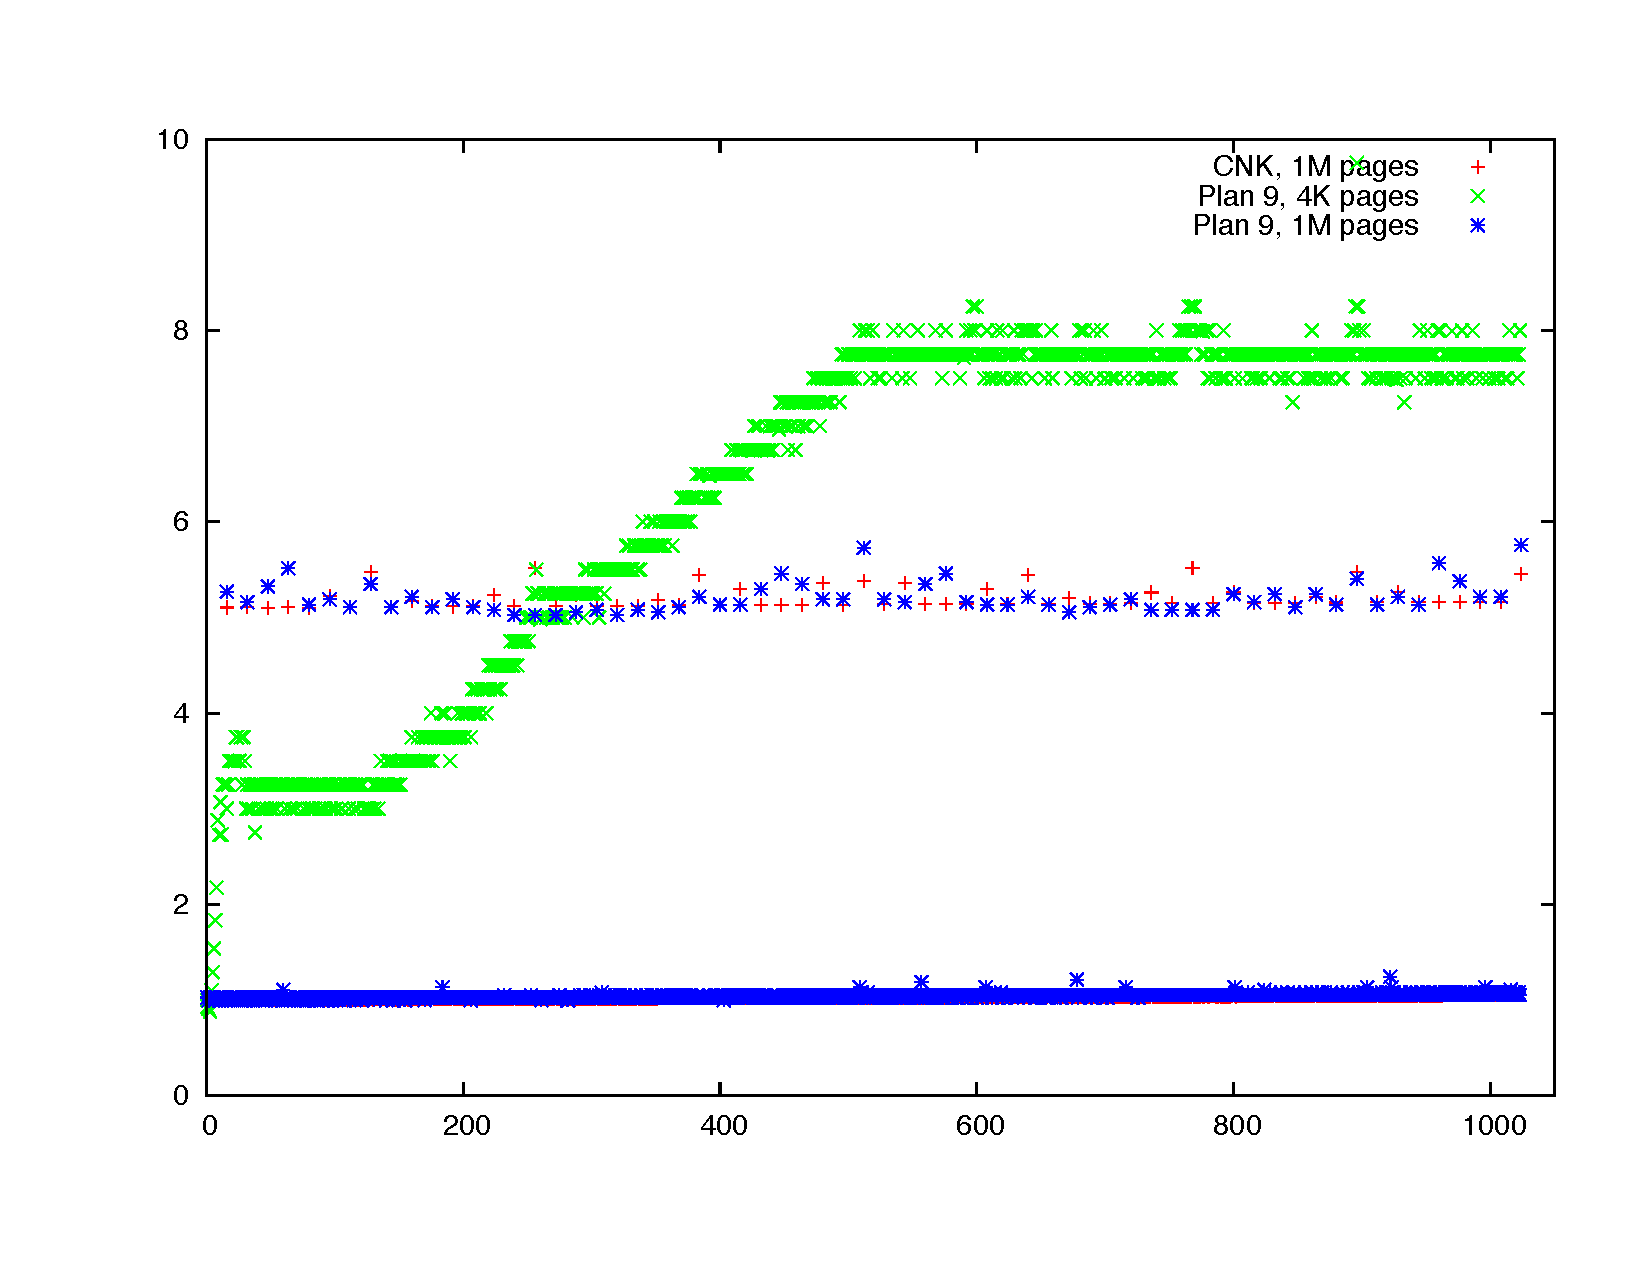
\includegraphics[width=4in]{strid3.pdf}
 \caption{{\bf Result of running strid3 on CNK, Plan 9, and Plan 9 with 1 MByte pages. }}
\label{strid3}
\end{center}
\end{figure}
to show the impact of TLB size upon an application. Shown in Figure \ref{strid3} is the result. Plan~9 is 
eight times slower than the CNK when 4096 byte pages are used. With one Mbyte pages in Plan~9, its 
performance is identical to the CNK. 
The change to Plan~9 to support the larger pages amounted to less than 30 lines of code\cite{DBLP:journals/ife/MinnichM09}. 

\subsection{Shared Heap}
\subsection{Currying}
\section{File Systems}
\subsection{Compute Node Caches}
\section{New network communications models}
\subsection{Active Message Support}
\subsection{What are we calling Charles stuff?}
\section{Kittyhawk Linux Kernel}
\subsection{Hybrid Networks}
\subsection{Communication Domains}
\subsection{Heterogenous Compute Node Kernels}
\section{Kittyhawk L4 Kernels}
\subsection{Virtual Machine Monitor for BG/P}
